\documentclass{segabs}

\usepackage{color}
\usepackage{array}
\usepackage{amsmath}
\usepackage{amssymb}
\usepackage{amsfonts}
\usepackage{amsthm}
\usepackage{mathtools}
\usepackage{relsize}
\usepackage{bm}
\usepackage{mleftright}

\setfigdir{Fig}
\usepackage{epstopdf}
\epstopdfsetup{outdir=./Fig/}

\newcommand{\Lorig}{\mathcal{L}}
\newcommand{\Lext}{\mathbf{L}}
\newcommand{\bvec}{\mathbf{b}}
\newcommand{\dtime}{\Delta t}
\newcommand{\dfreq}{\Delta \omega}
\newcommand{\A}{\mathbf{A}}
\newcommand{\B}{\mathbf{B}}
\newcommand{\Ainv}[1]{\mathbf{A}_{#1}^{-1}}
\newcommand{\Astarinv}[1]{{\mathbf{A}_{#1}^{\ast}}^{-1}}
\newcommand{\Lamb}{\bm{\Lambda}}
\newcommand{\D}{\mathbf{D}}
\newcommand{\I}{\mathbf{I}}
\newcommand{\M}{\mathbf{M}}
\newcommand{\Pbold}{\mathbf{P}}
\newcommand{\Lbold}{\mathbf{L}}
\newcommand{\Ubold}{\mathbf{U}}
\newcommand{\Gam}{\bm{\Gamma}}


\newcommand{\Rsamp}{\mathbf{R}}
\newcommand{\uorig}{\mathbf{u}}
\newcommand{\dvorig}{\delta \mathbf{v}}
\newcommand{\uext}{\delta \mathbf{u}}
\newcommand{\dorig}{\mathbf{d}}
\newcommand{\corig}{\mathbf{c}}
\newcommand{\dmorig}{\delta \mathbf{m}}
\newcommand{\cext}{\delta \mathbf{c}}
\newcommand{\src}{\mathbf{f}}
\newcommand{\pos}{\mathbf{x}}
\newcommand{\dpos}{\Delta \mathbf{x}}

\newcommand{\uorigh}{\hat{\mathbf{u}}}
\newcommand{\uexth}{\delta \hat{\mathbf{u}}}
\newcommand{\dvorigh}{\delta \hat{\mathbf{v}}}
\newcommand{\dorigh}{\hat{\mathbf{d}}}
\newcommand{\residh}{\hat{\mathbf{r}}}
\newcommand{\cexth}{\delta \hat{\mathbf{c}}}
\newcommand{\srch}{\hat{\mathbf{f}}}

\begin{document}

\title{Illumination compensation of shadow zones in extended least squares migrated images by solving the linear inverse problem in tomographic full waveform inversion}

\author{Rahul Sarkar, Stanford University, and Biondo Biondi, Stanford University}

\righthead{Illumination compensation by solving the TFWI linear inverse problem}

\maketitle

\vspace*{-0.7cm}
\begin{abstract}

\vspace*{-0.6cm}
Many different factors such as sub-optimal acquisition design or rapidly changing velocity profiles can contribute to the formation of shadow zones in migrated images, or more generally in least squares migrated images. The solution of tomographic full waveform inversion (TFWI) using the variable projection technique leads to a linear least squares inverse problem. For a fixed background model, solving this problem is equivalent to performing regularized extended least squares migration. We show in this abstract that the frequency domain formulation of the linear inverse problem makes this connection even more apparent and straightforward. We then demonstrate that in the Born scattering regime, the solution to this problem can be used as a tool to compensate for the lack of illumination in shadow zones, and hence remove illumination artifacts from least squares migrated images, including the extended case. Our claims are backed up using 2D numerical examples, where in the first example we correct for illumination artifacts caused only by a low velocity anomaly, while in the second example we additionally remove the effect of acquisition holes. We thus discover an interesting application of TFWI in the regime of linearized waveform inversion, where the goal is the estimation of the reflectivity component only, and not the full velocity model.
\end{abstract}
\vspace*{-0.7cm}
\section{Introduction}

The presence of shadow zones and illumination variability is an extremely common occurrence in seismic images, irrespective of whether they are obtained by Kirchhoff migration, reverse time migration (RTM) \citep{baysal1983reverse}, or more generally least squares migration (LSM) \citep{nemeth1999least, ronen2000least, dai2012multi}. Of course the choice of the migration algorithm impacts the severity of the phenomenon --- in general the effects are the greatest for ray based methods, and gets progressively better as one moves to wave equation based methods, and wave equation based least squares migration methods. However none of these algorithms can completely eliminate the phenomenon. The most common cause of shadow zones and illumination variability is poor acquisition design that lead to an uneven fold of coverage, and the formation of acquisition holes in azimuths, offsets and angles. Additionally, intrinsic factors such as rapidly changing velocity profiles could also lead to this phenomenon, for example such effects are extremely common in areas with very complex salt body geometries.

Other than the choice of the migration algorithm, mitigation strategies for acquisition related illumination artifacts involve techniques like pre-processing the data to interpolate missing traces, and normalizing the trace amplitudes based on fold. However uneven (or no) illumination caused by complex velocity models is much harder to compensate using these simple methods, and one must use regularization schemes instead. These regularization strategies are most easily implemented in the context of LSM, and our focus in this abstract will be on their wave equation variants. The use of regularizers for LSM is not new --- it has been applied to remove the effect of acquisition footprints from the image due to missing data \citep{nemeth1999least}, and it can be additionally used to further suppress cross-talk and missing data artifacts in LSM imaging of blended data \citep{tang2009least, xue2015seismic}. In the context of subsalt imaging, where illumination compensation is particularly challenging, a typical idea is to perform LSM along an extended axis and regularize the image along it, as has been done for example using geophysical regularizers along the offset ray parameter axis (or equivalently angles), and using steering filters \citep{prucha2002subsalt, clapp2005imaging, clapp2005regularized, kuehl2001generalized}. It should be noted that even with perfect acquisition, in areas with rapidly changing velocities, shadow zones tend to be the most prominent in the high frequency regime where wave propagation is well approximated by high frequency asymptotics, i.e. ray theory.

Tomographic full waveform inversion (TFWI) \citep{biondi2012tomographic, biondi2013tomographic, TFWI.gp} was originally developed as a heuristic method to mitigate some of the effects of cycle skipping that adversely affect the convergence of full waveform inversion (FWI). It belongs to a general class of methods, all of which are based on the idea of model extension --- the most notable examples being extension in subsurface offset or angle \citep{sava2003angle, rickett2002offset}, source extension \citep{huang2015full, huang2016matched}, and extension in time lag as in the case of TFWI. While several different strategies have been suggested to speed up the convergence of TFWI, such as wavelength continuation and scale separation \citep{almomin2012tomographic, almomin2013tomographic}, it was recently noted that the method of variable projection could be applied to solve the TFWI problem \citep{barnier2018full}, within a broader scheme of methods called full waveform inversion by model extension (FWIME). In this approach, at every iteration one fixes the physical velocity model, and solves a linear least squares optimization problem to obtain a solution for the extended model that minimizes the TFWI objective function. We will refer to this problem as the \textit{``TFWI linear inverse problem''}.

In this abstract, we will show that the frequency domain formulation of the TFWI linear inverse problem is equivalent to regularized extended LSM (with a specific choice of regularizer) along the extended frequency axis, which is simply the Fourier dual of the extended time lag axis. Because of the form of the objective function, we will additionally demonstrate a certain form of equivalence (to be made precise in the next section) with non-extended LSM. Using simple numerical examples, we will demonstrate how this formalism can be used to remove the effect of illumination artifacts in migrated images or extended migrated images, that arise either due to the complexity of the velocity model or from acquisition holes.
\vspace*{-0.8cm}
\section{Theory}

\vspace*{-0.2cm}
\subsection{Setup of the TFWI linear inverse problem}

\vspace*{-0.1cm}
The frequency domain formulation of the TFWI linear inverse problem and an efficient solution strategy to solve it has been developed in \cite{Sarkar.sep.172.rahul1}. The formulation leads to the problem of minimization of the linear least squares objective function $\hat{J}(\cexth)$ given by the expression

\vspace*{-0.7cm}
\begin{equation}
\sum_{k=1}^{N_\omega} \sum_{i=1}^{N_s} ||\Rsamp_i \uexth_{ki} - \residh_{ki}||_2^2 + \epsilon^2 \left\lVert\; \frac{\partial}{\partial \omega} \cexth \right\rVert^2_2 + \gamma^2 ||\cexth||^2_2\;,
\label{eq:Jtfwi-mod-freq}
\end{equation}
\vspace*{-0.5cm}

that needs to be solved at every iteration inside a variable projection scheme for a fixed value of the physical velocity model $\corig$, with the goal of obtaining $\cexth^{\ast}$ that minimizes \eqref{eq:Jtfwi-mod-freq}. The expression above is readily obtained from the original time domain TFWI objective function \citep{TFWI.gp}, with the only exception of the $||\cexth||_2$ term which has been added to make the linear inverse problem well-posed, by Fourier transforming all quantities in time and by using the fact that the Fourier transform preserves the $L^2$ norm. In expression \eqref{eq:Jtfwi-mod-freq}, $\epsilon, \gamma \in [0, \infty)$, $N_\omega$ and $N_s$ are the number of discrete frequencies and sources in the inversion respectively, and $\cexth$ is the frequency domain extended model. For the $i^{th}$ source and $k^{th}$ frequency, $\Rsamp_i$ denotes the restriction operator that samples the wave field at the receiver locations, $\residh_{ki} = \dorigh_{ki} - \Rsamp_i \uorigh_{ki}$ where $\dorigh_{ki}$ represents the recorded data, and $\uorigh_{ki}, \uexth_{ki}$ represents the physical wave field and the extended Born modeled wave field respectively, obtained by solving the following system of Helmholtz equations for angular frequency $\omega_k$ and source function $\srch_{ki}$:

\vspace*{-0.6cm}
\begin{equation}
\begin{split}
& \left( \mathbf{\nabla}^2 + \omega_k^2 / \corig^2 \right) \uorigh_{ki} = - \srch_{ki} \;,\\
& \left( \mathbf{\nabla}^2 + \omega_k^2 / \corig^2 \right) \uexth_{ki} = \left( 2 \omega_k^2 / \corig^3 \right) \uorigh_{ki} \cexth_{k} \;.
\end{split}
\label{eq:upde-helmholtz}
\end{equation}
\vspace*{-0.6cm}

In the second equation in \eqref{eq:upde-helmholtz}, $\cexth_{k}$ represents the component of $\cexth$ corresponding to the $k^{th}$ frequency. Discretizing \eqref{eq:Jtfwi-mod-freq} on a spatial grid leads to the linear least squares problem of minimizing the objective function (still denoted as $\hat{J}(\cexth)$)

\vspace*{-0.7cm}
\begin{equation}
\sum_{k=1}^{N_\omega} \sum_{i=1}^{N_s} ||\Rsamp_i \uexth_{ki} - \residh_{ki}||_2^2 + \epsilon^2 \left\lVert\; \D \cexth \right\rVert^2_2 + \gamma^2 ||\cexth||^2_2\;,
\label{eq:Jtfwi-freq-discrete}
\end{equation}
\vspace*{-0.5cm}

where all quantities now represent their discrete equivalents, and we take $\D$ to be the forward difference derivative operator acting along the frequency axis.

In the next subsections, we will show the connection of \eqref{eq:Jtfwi-freq-discrete} with regularized LSM and extended LSM, but for this we will assume that we are in the Born scattering regime, i.e. the physical velocity $\corig$ is a reasonably good approximation of the smooth background velocity model, so that $\residh_{ki}$ is well approximated by first order Born scattering. Notice that in this regime, if $\dmorig$ represents the perturbation in the physical velocity (independent of frequency), then the Born scattered wave field $\dvorigh_{ki}$, for the $i^{th}$ source and $k^{th}$ frequency, is given by (note the resemblance with the second equation in \eqref{eq:upde-helmholtz})

\vspace*{-0.4cm}
\begin{equation}
\left( \mathbf{\nabla}^2 + \omega_k^2 / \corig^2 \right) \dvorigh_{ki} = \left( 2 \omega_k^2 / \corig^3 \right) \uorigh_{ki} \dmorig \;.
\label{eq:born-helmholtz}
\end{equation}
\vspace*{-0.5cm}

\subsection{Relation to regularized extended LSM}

\vspace*{-0.1cm}
The general form of regularized extended LSM in the frequency extended space (the same form is valid in any extended domain) is given by the minimization of any objective function of the form

\vspace*{-0.6cm}
\begin{equation}
\Phi(\cexth) = \sum_{k=1}^{N_\omega} \sum_{i=1}^{N_s} ||\Rsamp_i \uexth_{ki} - \residh_{ki}||_2^2 + \epsilon^2 \left\lVert\; \A \cexth \right\rVert^2_2 \;,
\label{eq:Jextreg}
\end{equation}
\vspace*{-0.4cm}

where $\A$ is a linear operator. We will not consider non-linear regularization as they are not common in seismic imaging applications. Notice that $\uexth_{ki}$ depends linearly on $\cexth_k$ by \eqref{eq:upde-helmholtz}, and thus \eqref{eq:Jextreg} is indeed a linear least squares problem. The interpretation is simple --- the first term is the data fitting term that seeks to find $\cexth_k$ that minimizes the data misfit for the $k^{th}$ frequency, while the second term is the regularization term that constrains the relationship between the different $\cexth_k$'s. Thus \eqref{eq:Jtfwi-freq-discrete} can be put in the form of \eqref{eq:Jextreg} by simply noting that

\vspace*{-0.5cm}
\begin{equation}
\epsilon^2 \left\lVert\; \D \cexth \right\rVert^2_2 + \gamma^2 ||\cexth||^2_2 \; = \; \left| \left| \; 
\begin{bmatrix}
\epsilon \D \\
\gamma \I
\end{bmatrix}
\cexth \; \right| \right|_2^2 \;.
\label{eq:Jextreg_relation}
\end{equation}
\vspace*{-0.5cm}

\subsection{Relation to regularized LSM}

\vspace*{-0.1cm}
The relationship with regularized LSM is only slightly more difficult to establish. Similar to \eqref{eq:Jextreg}, the general form of regularized LSM is given by the minimization of any objective function of the form

\vspace*{-0.7cm}
\begin{equation}
\Psi(\dmorig) = \sum_{k=1}^{N_\omega} \sum_{i=1}^{N_s} ||\Rsamp_i \dvorigh_{ki} - \residh_{ki}||_2^2 + \eta^2 \left\lVert\; \A \dmorig \right\rVert^2_2 \;,
\label{eq:Jlsmreg}
\end{equation}
\vspace*{-0.5cm}

and the key difference compared to \eqref{eq:Jextreg} is that the minimization is now over the velocity perturbation $\dmorig$, which is purely in the physical space. Again by \eqref{eq:born-helmholtz} it is clear that \eqref{eq:Jlsmreg} represents a linear least squares problem. To establish the relationship with \eqref{eq:Jtfwi-freq-discrete}, let us first rewrite minimization of \eqref{eq:Jlsmreg} in the equivalent form

\vspace*{-1.0cm}
\begin{equation}
\begin{split}
& \text{minimize} \;\;\;\; \sum_{k=1}^{N_\omega} \sum_{i=1}^{N_s} ||\Rsamp_i \uexth_{ki} - \residh_{ki}||_2^2 + \frac{\eta^2}{N_\omega} \left\lVert\; (\I_{N_\omega} \otimes \A) \cexth \right\rVert^2_2 \\
& \text{subject to} \;\;\;\;\; \D \cexth = 0.
\end{split}
\label{eq:Jlsmreg-eqv}
\end{equation}
\vspace*{-0.7cm}

In the above expression $\otimes$ denotes the Kronecker product, $\I_{N_\omega}$ is the identity matrix of size $N_\omega \times N_\omega$, and the constraint simply expresses the condition $\cexth_{1} = \dots = \cexth_{N_\omega}$, as $\D$ is the forward difference derivative operator. One should also note that \eqref{eq:Jlsmreg-eqv} is equivalent to \eqref{eq:Jlsmreg} only because the second equation in \eqref{eq:upde-helmholtz}, and \eqref{eq:born-helmholtz} are functionally similar to one another, only differing in the right hand side ($\cexth_{k}$ vs $\dmorig$). It then follows from well known properties of the quadratic penalty method, that if one considers the family of unconstrained minimization problems (parameterized by $\epsilon$) with objective functions

\vspace*{-0.7cm}
\begin{equation}
\sum_{k=1}^{N_\omega} \sum_{i=1}^{N_s} ||\Rsamp_i \uexth_{ki} - \residh_{ki}||_2^2 + \epsilon^2 ||\D \cexth||_2^2 + \frac{\eta^2}{N_\omega} \left\lVert\; (\I_{N_\omega} \otimes \A) \cexth \right\rVert^2_2 \;,
\label{eq:Jlsmreg-eqv-uncons}
\end{equation}
\vspace*{-0.7cm}

such that $\epsilon \rightarrow \infty$, and $\pos_\epsilon$ is a global minimizer of \eqref{eq:Jlsmreg-eqv-uncons} at parameter value $\epsilon$, then if $\pos^{\ast}$ is any limit point of the sequence $\{ \pos_\epsilon \}$, $\pos^{\ast}$ is also a global minimizer of the constrained problem \eqref{eq:Jlsmreg-eqv} (see Theorem 17.1 in \cite{nocedal2006numerical}), and hence of \eqref{eq:Jlsmreg}. It is clear that \eqref{eq:Jtfwi-freq-discrete} is a special case of \eqref{eq:Jlsmreg-eqv-uncons} when $\A = \I$, and $\gamma = \eta / \sqrt{N_\omega}$. To make this work, in principle one should gradually increase $\epsilon$ and solve \eqref{eq:Jlsmreg-eqv-uncons} repeatedly, till the resulting minimizers converge. However this is not possible in practice as solving \eqref{eq:Jlsmreg-eqv-uncons} is expensive. An alternative strategy is to simply choose a large value of $\epsilon$ (which can be done with a few finite number of trials), and solve \eqref{eq:Jtfwi-freq-discrete} for this $\epsilon$ to get $\cexth^{\ast}$, and then get an estimate of the optimal $\dmorig^{\ast}$ by averaging

\vspace*{-0.5cm}
\begin{equation}
\dmorig^{\ast} = \frac{1}{N_\omega} \sum_{k=1}^{N_\omega} \cexth_{k}^{\ast} \;,
\label{eq:dmavg}
\end{equation}
\vspace*{-0.5cm}

where we have assumed that the inversion is performed over the same positive and negative frequencies, and so $\dmorig^{\ast}$ is real valued, because if $\cexth_{k}^{\ast}$ is the solution for any positive frequency, then $\overline{\cexth_{k}^{\ast}}$ is the solution for the corresponding negative frequency. In practice to reduce the computational cost by a factor of two, one can simply perform the inversion over the positive frequencies, and set the $\cexth^{\ast}_k$'s corresponding to the negative frequencies according to this relation. In what follows, we will refer to $\dmorig^{\ast}$ obtained this way to be the \textit{stacked inverted image}.
\vspace*{-0.4cm}
\section{Numerical Examples}
\vspace*{-0.2cm}
All the numerical experiments in this section are run for models of size 3 km $\times$ 2 km in the X and Z directions respectively, with a 5 m $\times$ 5 m grid spacing. Sources are placed every 50 m on the surface. The inversion is performed over the frequency band $6.67 \; \text{Hz} \leq \omega / 2 \pi \leq 30 \; \text{Hz}$, which is uniformly divided into $N_\omega = 50$ discrete frequencies. We use a Gaussian spectrum for the source wavelet (in the frequency domain), centered at 18 Hz with a standard deviation of 7 Hz. In addition we apply a linear taper (decaying to zero) on either side of the spectrum between 6.67 - 9 Hz, and 27.67 - 30 Hz. The TFWI linear inverse problem is solved in each case using the method outlined in \cite{Sarkar.sep.172.rahul1}, and for simplicity we set $\gamma = 0$ in all the tests.

\vspace*{-0.4cm}
\begin{figure}[h]
\centering
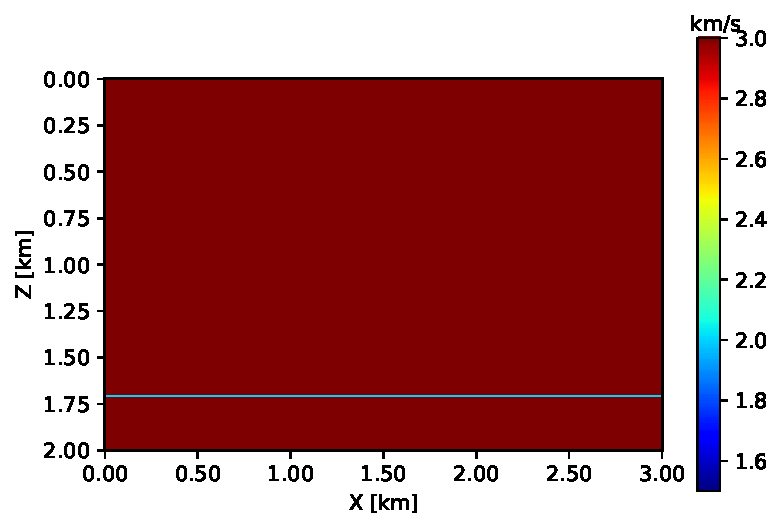
\includegraphics[width=0.8\linewidth]{Fig/veltrue-noanomaly.pdf}

\vspace*{-0.4cm}
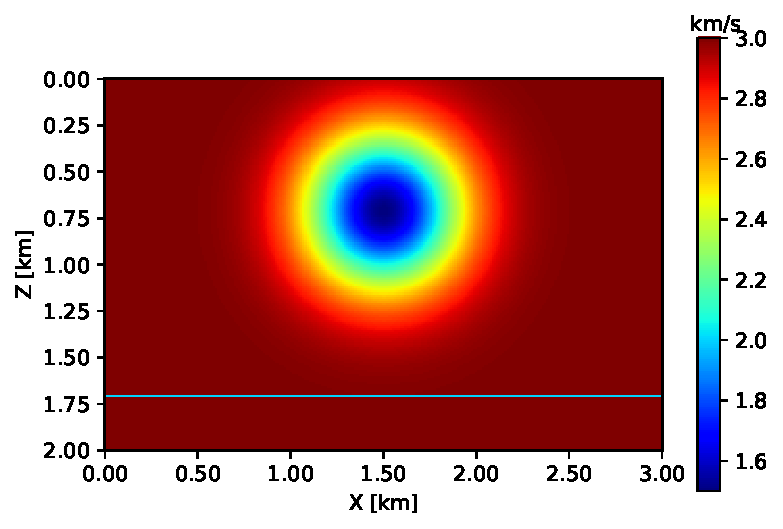
\includegraphics[width=0.8\linewidth]{Fig/veltrue-anomaly.pdf}

\vspace*{-0.5cm}
\caption{Background models without (top) and with low velocity Gaussian anomaly (bottom). The reflector is overlain at a depth of 1.71 km.}
\label{fig:example1_models}
\end{figure}

\subsection{Illumination compensation for a low velocity anomaly}

\vspace*{-0.1cm}
In the first example, we consider two cases corresponding to the models shown in Figure \ref{fig:example1_models}, one of which contains a low velocity Gaussian anomaly, and the other one has a constant velocity of 3 km/s. The reflector is placed in both cases at a depth of 1.71 km (which is overlain on the figure), and used to generate the Born data $\residh_{ki}$ with a split spread acquisition geometry, and maximum offset of 2 km. The displayed models (without the displayed reflector) form the background velocities for the linear inversion. 

\vspace*{-0.3cm}
\begin{figure}[h]
\centering
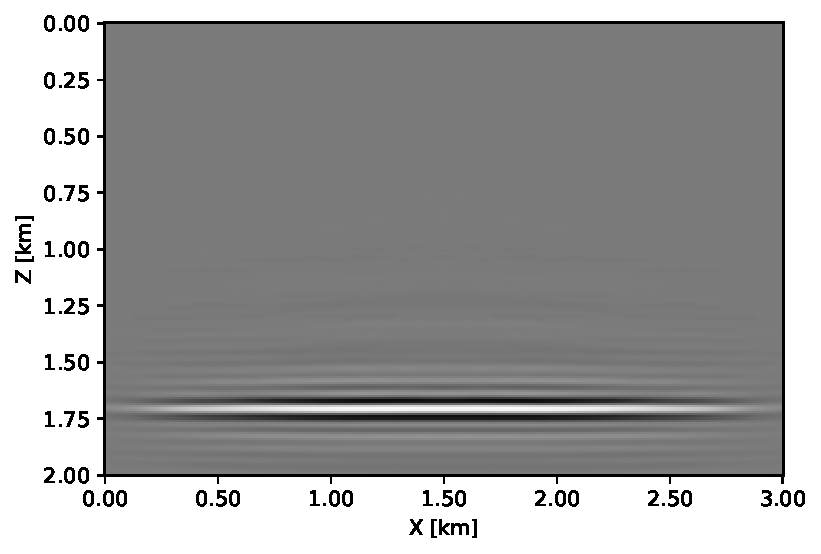
\includegraphics[width=0.7\linewidth]{Fig/noanomaly-inverted-image-stack.pdf}

\vspace*{-0.3cm}
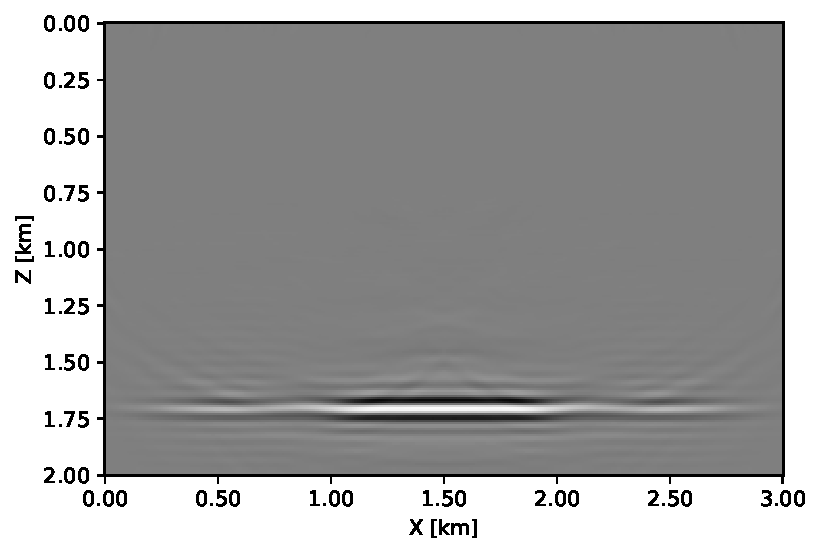
\includegraphics[width=0.7\linewidth]{Fig/anomaly-inverted-image-stack.pdf}

\vspace*{-0.5cm}
\caption{Stacked inverted images $\dmorig^{\ast}$ without regularization ($\epsilon = 0$) for the constant velocity model (top), and the low velocity Gaussian anomaly model (bottom).}
\label{fig:example1_stacks_noreg}
\end{figure}
\vspace*{-0.3cm}
\begin{figure}[h]
\centering
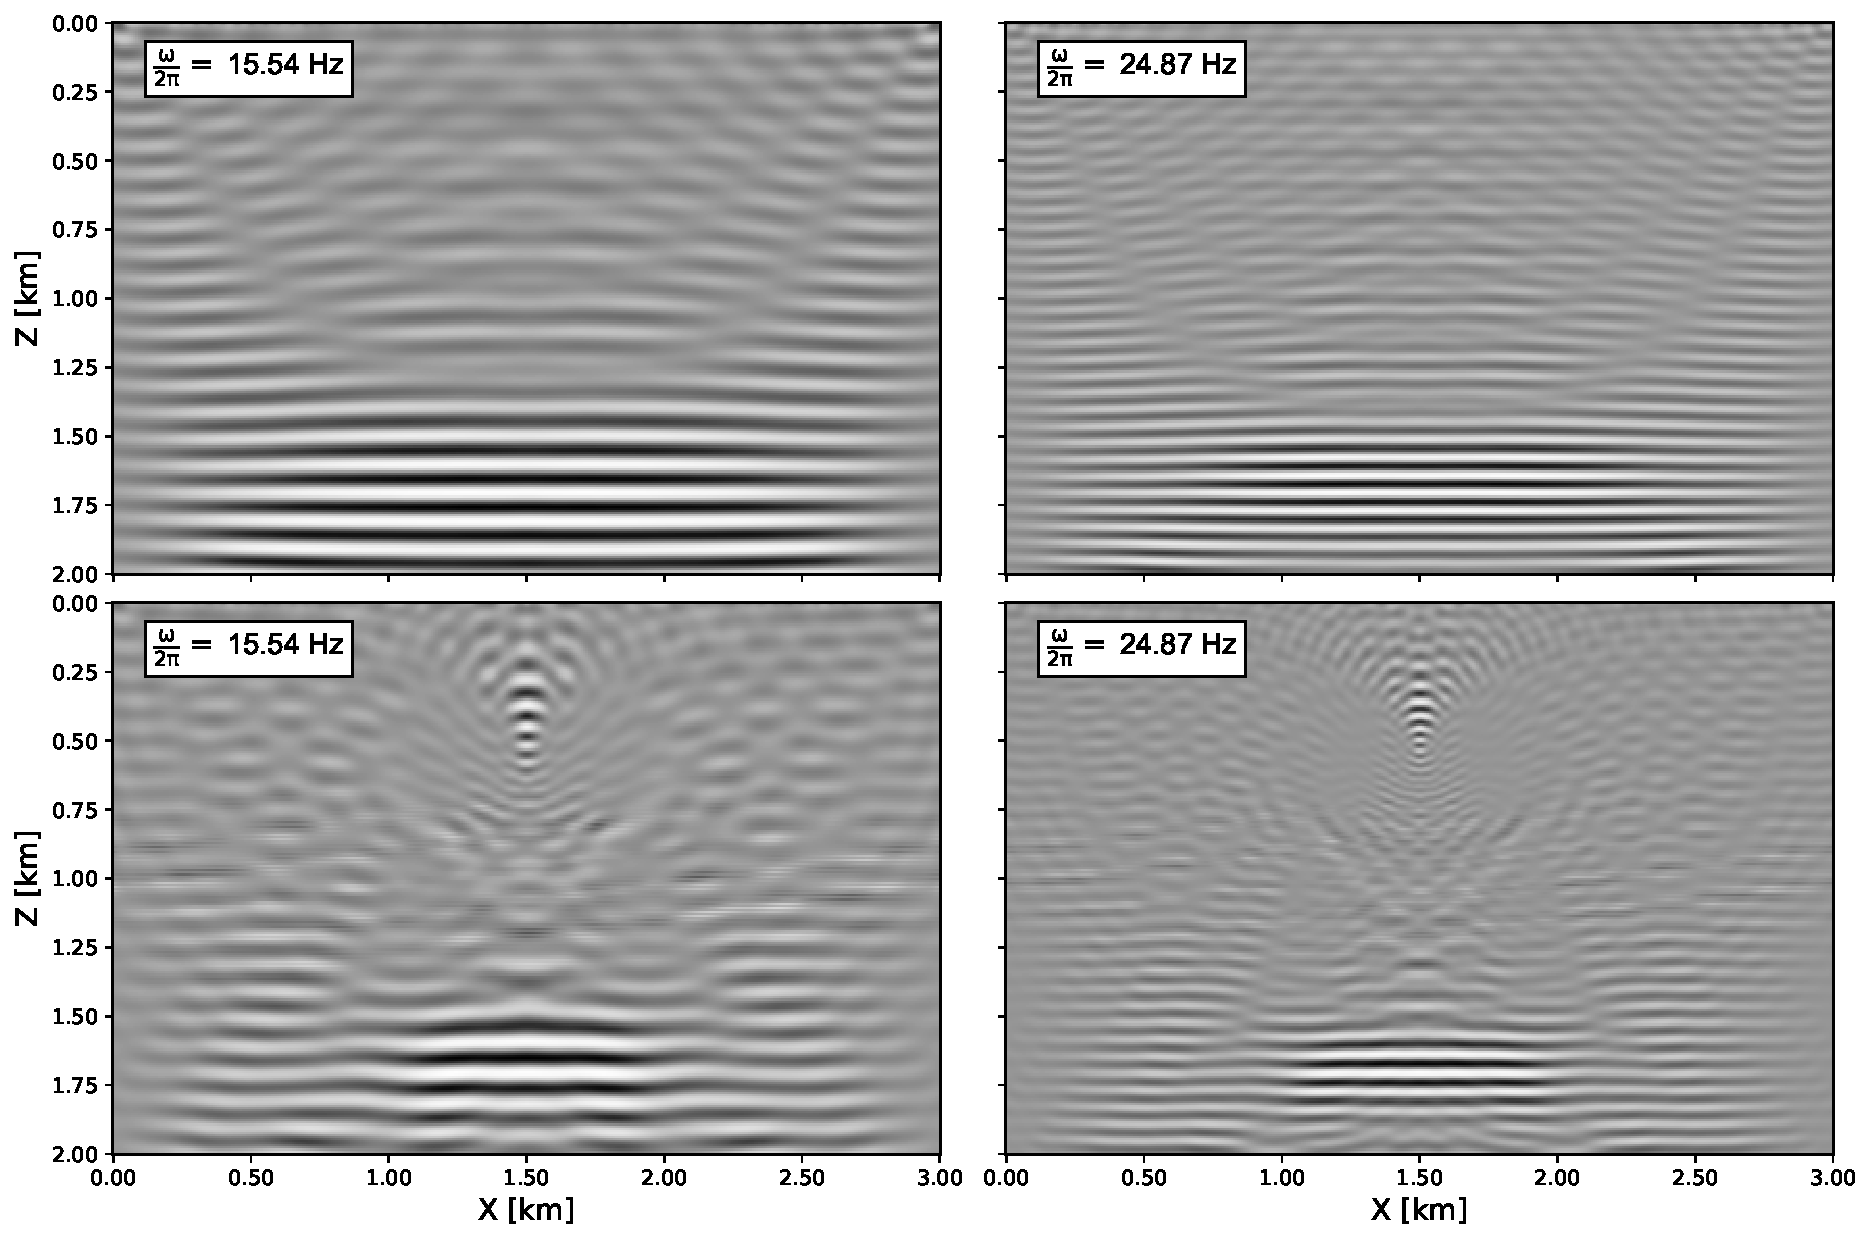
\includegraphics[width=\linewidth]{Fig/inverted-images-noreg-comparison.pdf}

\vspace*{-0.4cm}
\caption{Real parts of the inverted images $\cexth^{\ast}_k$ without regularization ($\epsilon = 0$) for the constant velocity model (top row), and the low velocity Gaussian anomaly model (bottom row). The columns correspond to $k = 20,\; \omega / 2 \pi = 15.54$ Hz (left), and $k = 40,\; \omega / 2 \pi = 24.86$ Hz (right).}
\label{fig:example1_noreg_comp}
\end{figure}

\vspace*{-0.3cm}
We first solve the linear inverse problem in both cases without any regularization ($\epsilon = 0$). The stacked inverted images for the two cases are shown in Figure \ref{fig:example1_stacks_noreg}, and the inverted images $\cexth_{k}^{\ast}$ for $k=20$ and $k=40$, corresponding to the frequencies of 15.54 Hz and 24.87 Hz respectively, are shown in Figure \ref{fig:example1_noreg_comp}. In Figure \ref{fig:example1_noreg_comp}, we have only displayed the real parts of $\cexth_{k}^{\ast}$ due to space constraints, but the imaginary parts also have similar behavior. It is clear from these illustrations that the inverted images for the Gaussian anomaly have shadow zones at some offset from the center of the model on either side, and this effect gets more prominent at larger frequencies. In fact at the reflector level, the amplitudes decrease and then increase again as one moves either to the right or to the left from the center, an effect that is most easily seen in the stacked inverted image (Figure \ref{fig:example1_stacks_noreg}). The images corresponding to the constant velocity case do not exhibit these effects, and hence we can conclude that the complexity of the background model alone causes the uneven illumination at the reflector level for the low velocity Gaussian anomaly model.

\vspace*{-0.1cm}
\begin{figure}[h]
\centering
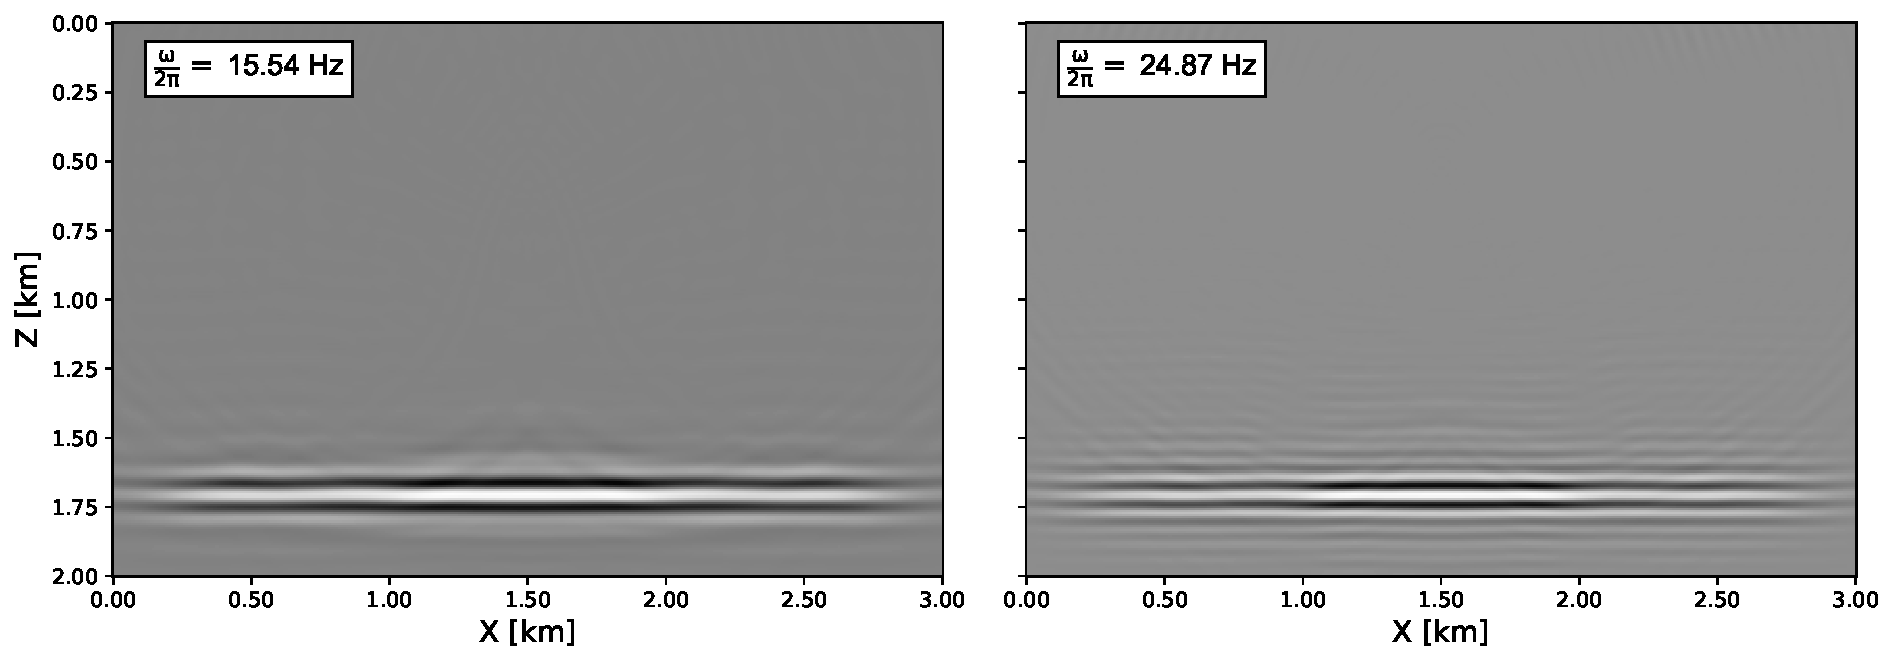
\includegraphics[width=\linewidth]{Fig/inverted-images-reg-anomaly.pdf}

\vspace*{-0.5cm}
\caption{Real parts of the inverted images $\cexth^{\ast}_k$ with regularization ($\epsilon = 0.2$) for the low velocity Gaussian anomaly model. The images correspond to $k = 20,\; \omega / 2 \pi = 15.54$ Hz (left), and $k = 40,\; \omega / 2 \pi = 24.86$ Hz (right).}
\label{fig:example1_images_reg}
\end{figure}

\vspace*{-0.2cm}
\begin{figure}[h]
\centering
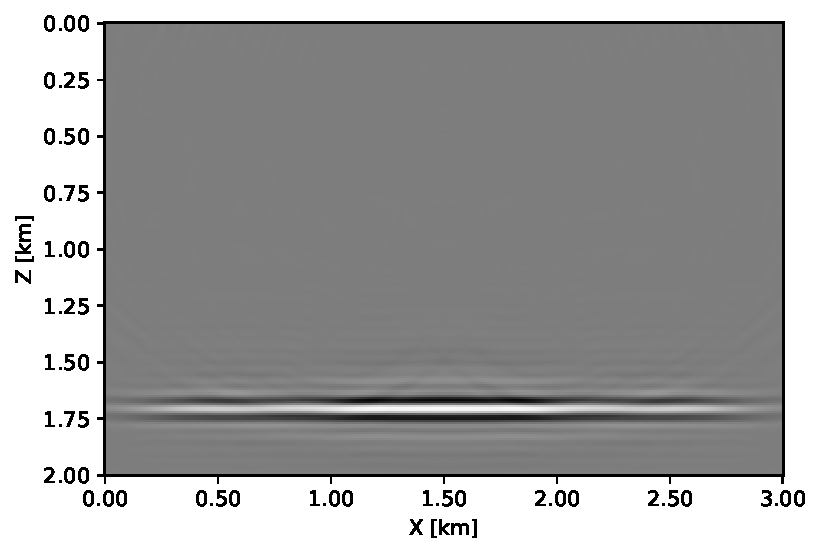
\includegraphics[width=0.7\linewidth]{Fig/anomaly-inverted-image-stack-reg.pdf}

\vspace*{-0.5cm}
\caption{Stacked inverted image $\dmorig^{\ast}$ with regularization  for the low velocity Gaussian anomaly model ($\epsilon = 0.2$).}
\label{fig:example1_stack_reg}
\end{figure}

\vspace*{-0.2cm}
We now show what happens when we turn on the regularization in the linear inversion, where after some tests the regularization strength was set at $\epsilon = 0.2$. In Figure \ref{fig:example1_stack_reg} we have displayed the stacked inverted image with the Gaussian anomaly model, while in Figure \ref{fig:example1_images_reg} the inverted images are shown at the same two frequencies as in Figure \ref{fig:example1_noreg_comp} to enable a direct comparison. We see that the effect of regularization is to ``equalize'' the inverted images, which is clearly seen in Figure \ref{fig:example1_images_reg} as the images tend to become similar to each other across frequencies. This is to be contrasted with the bottom-row images in Figure \ref{fig:example1_noreg_comp} where there is great variation between the images at the two frequencies with the same Gaussian anomaly model. The net effect of this phenomenon on the stacked inverted image in Figure \ref{fig:example1_stack_reg} is that in comparison to the bottom image in Figure \ref{fig:example1_stacks_noreg}, the reflector has been imaged more uniformly and continuously.

\subsection{Illumination compensation for a low velocity anomaly and acquisition hole}

\vspace*{-0.1cm}
In the second example we take exactly the same low velocity Gaussian anomaly model, the same reflector configuration, and the same acquisition configuration, except that all sources and receivers have been removed in a 0.5 km region, centered over the location of the Gaussian anomaly. In physical coordinates, this corresponds to the region $X = 1.25 - 1.75$ km. We again perform the same experiments --- solve the TFWI linear inverse problem with and without regularization. The value $\epsilon=0.2$ was chosen for the regularized inversion. The stacked inverted images for the two cases are displayed in Figure \ref{fig:example2_images_stacks}, while the inverted images are shown for the same two frequencies (as in the first example) for these cases in Figure \ref{fig:example2_image_comp}. Just like the first example, it is observed that the effect of the regularization term is to equalize the inverted images over frequencies, that leads to better continuity and illumination compensation of the reflector in the stacked inverted image.

\vspace*{-0.2cm}
\begin{figure}[h]
\centering
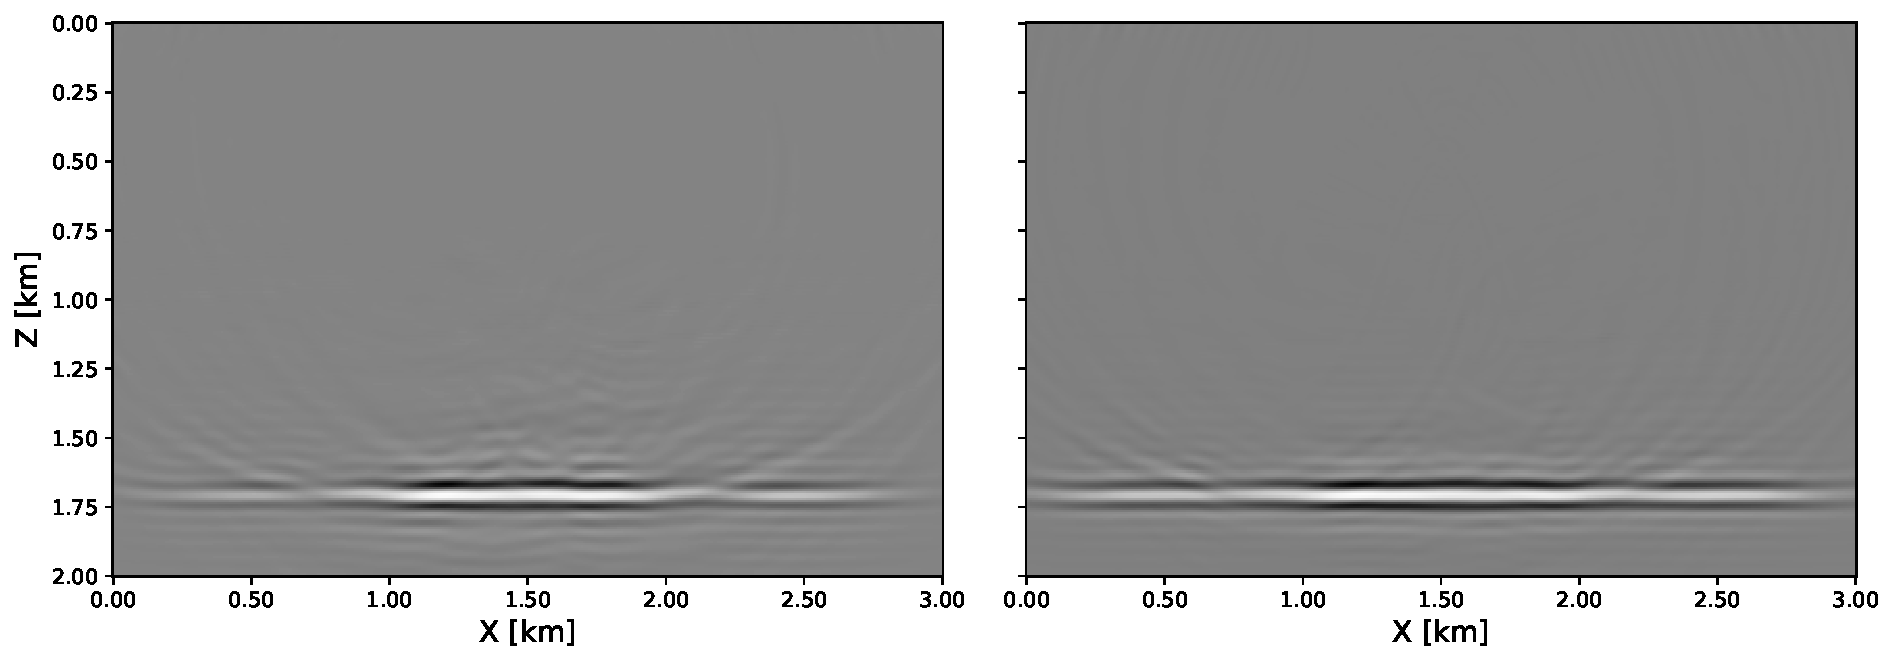
\includegraphics[width=\linewidth]{Fig/anomaly-hole-inverted-image-stack-comp.pdf}

\vspace*{-0.5cm}
\caption{Stacked inverted images $\dmorig^{\ast}$ with regularization (right), and without regularization (left) for the low velocity Gaussian anomaly model, in the presence of acquisition hole.}
\label{fig:example2_images_stacks}
\end{figure}
\vspace*{-0.2cm}
\begin{figure}[h]
\centering
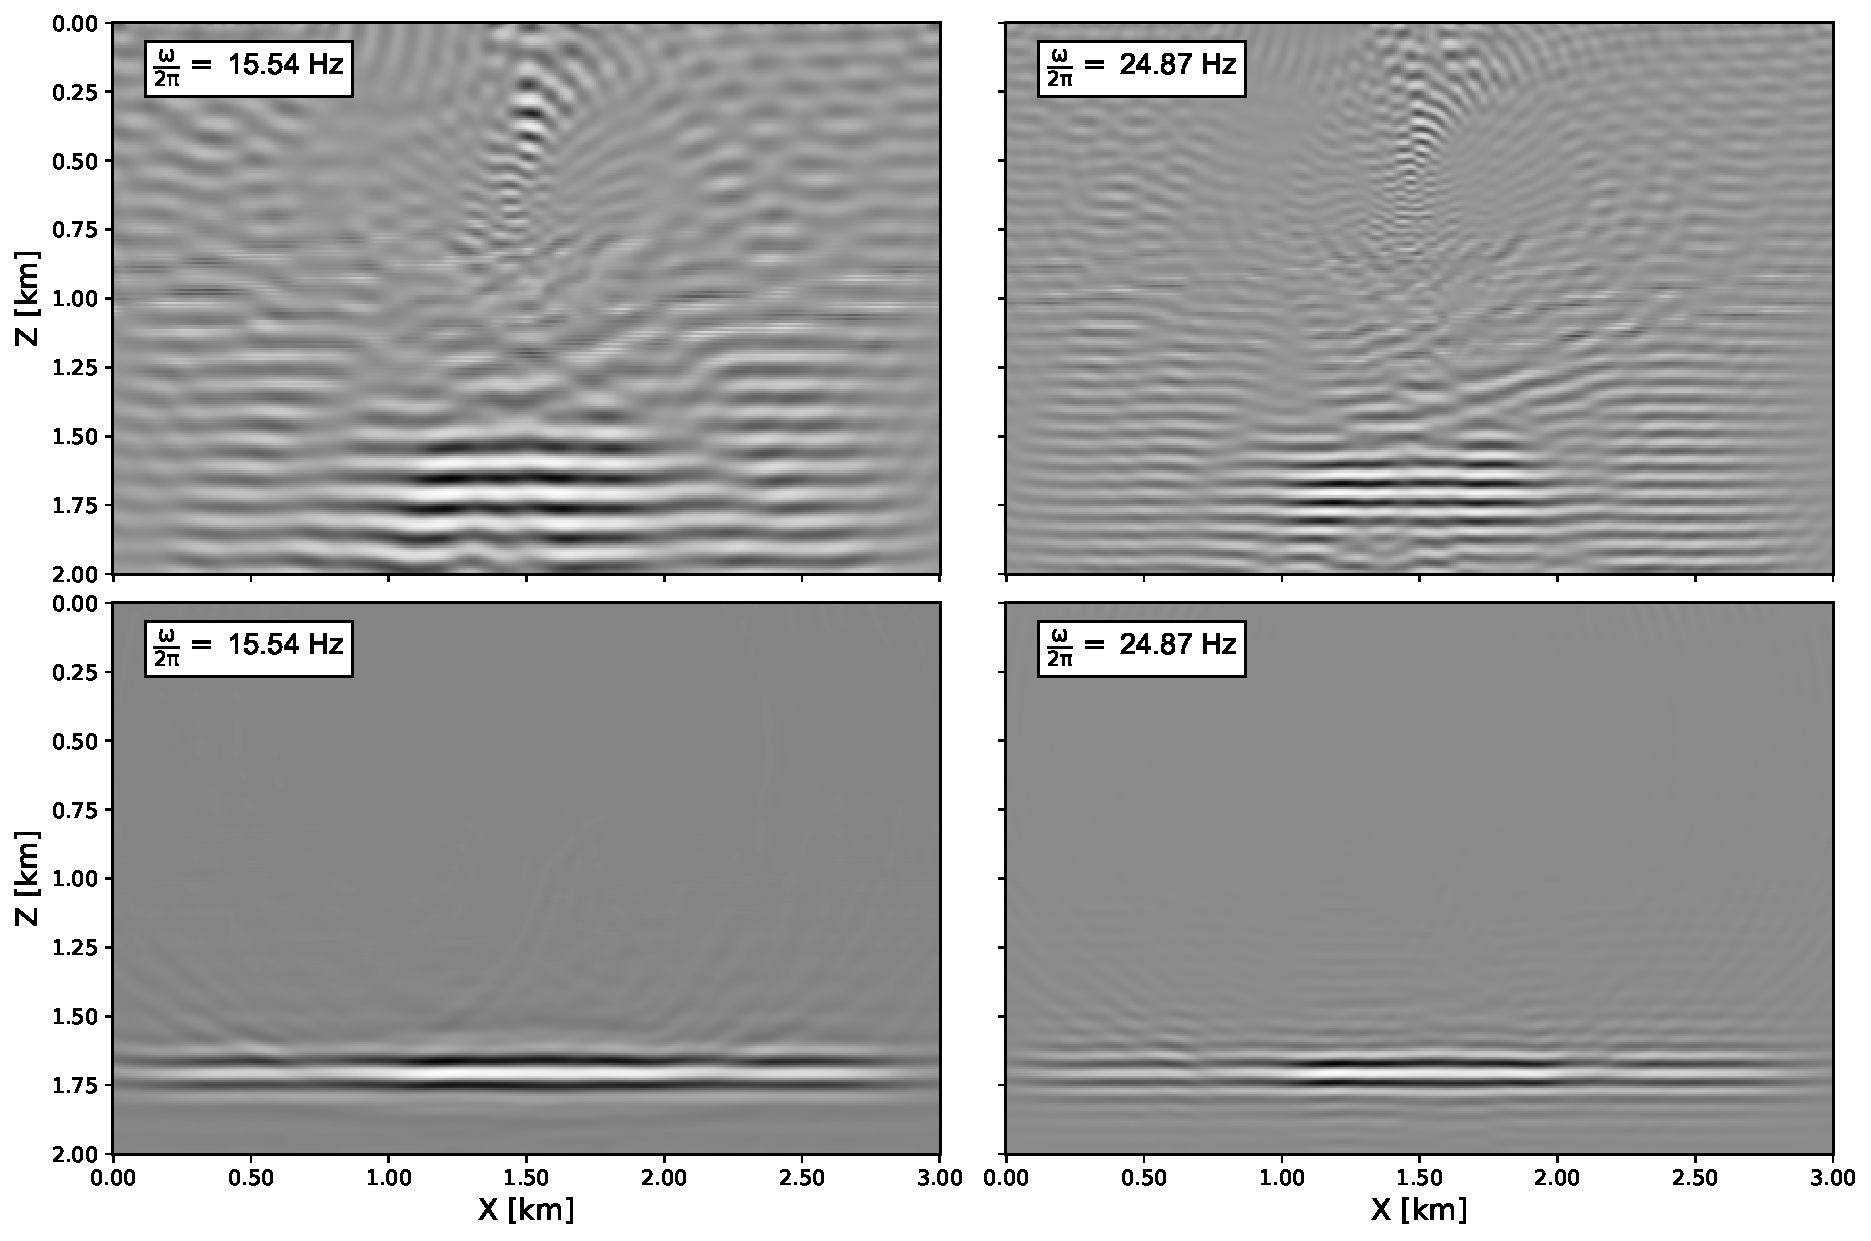
\includegraphics[width=\linewidth]{Fig/hole-inverted-images-comparison.pdf}

\vspace*{-0.4cm}
\caption{Real parts of the inverted images $\cexth^{\ast}_k$ in the presence of acquisition hole for the low velocity Gaussian anomaly model. The rows correspond to the cases without regularization (top), and with regularization (bottom). The columns correspond to $k = 20,\; \omega / 2 \pi = 15.54$ Hz (left), and $k = 40,\; \omega / 2 \pi = 24.86$ Hz (right).}
\label{fig:example2_image_comp}
\end{figure}
\vspace*{-0.6cm}
\section{Comments and Discussions}
\vspace*{-0.2cm}
The examples that we have shown are in 2D, but the conclusions are equally valid in the 3D setting; however solving the problem in 3D is not feasible at the moment for high frequencies using the direct factorization method of the Helmholtz equation that we are using. The parameter $\epsilon$, which controls the regularization strength, requires some tuning. We also know based on comprehensive numerical testing that the regularization scheme works well when the illumination holes are not very large; beyond which one begins to see artificial structures in the migrated image.
\vspace*{-0.4cm}
\section{Acknowledgments}
\vspace*{-0.2cm}
We would like to thank the affiliates of the Stanford Exploration Project for providing financial support for the duration of this study.

\twocolumn

\bibliographystyle{seg}  % style file is seg.bst
\bibliography{paper}

\end{document}
